% !TeX spellcheck = en_GB

\section{Accounting for Neural Nonlinearities}
\label{sec:recurrent_weights}

Minimising the linear quadratic loss in \cref{eqn:weight_optimise_currents_temporal} results in weights that---in some \emph{linear} networks (cf.~\Cref{sec:temporal_tuning_lti})---optimally realise \LTI systems while at the same time compensating for synaptic filters.
As we mentioned before, this focus on linear networks is not a major obstacle.
Linear activations can be emulated in networks of nonlinear neurons using \NEF identity decoders (cf.~\Cref{sec:nef_representation}).
Being able to do this is not just of theoretical interest. To the contrary, implementing linear dynamics on top of nonlinear networks is useful in practice.
As we discuss in \Cref{chp:cerebellum}, we can for example build an adaptive filter by transforming the state $\vec m(t)$ represented in the network.

Still, it can also be beneficial to solve for dense weight matrices that realise temporal tuning in networks of nonlinear neurons.
First and foremost, this allows modellers to finely control the temporal properties of individual neurons.
% and thus to model biological systems such as those described in \Cref{sec:temporal_tuning_biology}.
Furthermore, the temporal tuning curve paradigm suggests a natural way to represent multi-dimensional quantities over time.
Lastly, we can take heterogeneous synaptic filters into account, now at the level of individual synapses (cf.~\Cref{fig:nef_dynamics_neurons_b}).

In this section, we discuss solving for synaptic weights in nonlinear networks.
To this end, we propose a method for generating input signals $\mathfrak{x}_k$ that uniformly cover the neural activity space.
We then confirm in several experiments that our methods can be used to successfully build networks with the intended properties.
% TODO
%We then show how to account for the intrinsic dynamics of LIF neurons in low-firing rate regimes by estimating a temporal current-translation function.
%Finally, we use the techniques discussed here to construct adaptive filter that learns nonlinear dynamics.

\subsection{Sampling Input Signals and Temporal Encoders}
\label{sec:solve_dynamics_nonlinear_neurons}

On the surface, switching from linear units to neurons with nonlinear response curves, $G$, does not change our weight optimisation problem.
Recall that our least-squares loss was given as
\begin{align}
	E &= \sum_{k = 1}^N \left[
		J_i \left( \! \int_0^\infty \!\!\! \big\langle \mathfrak{e}_i(\tau), f(\mathfrak{x}_k \ast \delta_\tau) \big\rangle \, \mathit{d\tau} \right) \,\,-\,\,
		\sum_{j = 1}^m w_{ij} \! \int_0^\infty \!\!\! h_{ij}(\tau) a_j(\mathfrak{x}_k \ast \delta_\tau) \,\mathrm{d}\tau
	\right]^2 \,.
	\tag{\ref{eqn:weight_optimise_currents_temporal}}
\end{align}
In linear networks, the current-translation function $J_i$ and the pre-population tuning curve $\mathfrak{a}_j$ are linear.
While we continue to assume that $J_i$ is linear,%
\footnote{
Remember that we saw in \Cref{sec:nef_decode_current} that we can usually decode biases directly from the pre-population.
}
the tuning-curve $\mathfrak{a}_j$ is now nonlinear in $\mathfrak{x}_k$ due to the neural response curve $G$.
Additionally, each population now consists of hundreds of neurons, compared to the few dozen linear units in our above examples.

This poses two new challenges.
First, it is unclear how to assign temporal tuning curves to each neuron.
Before, we had a one-to-one mapping between linear units and the impulse responses of the \LTI system we wanted to realise; we now need to assign $q$ impulse responses to $n$ neurons, where typically $n \gg q$.
%For the orthonormal basis functions discussed above, $n$ must generally be much larger than $q$.
%We analysed this in \Cref{sec:dendritic_computation_theory_numerical}, where we saw that a relatively large number of neurons is required to span a separate orthogonal dimension.
Second, the selection of input signals $\mathfrak{x}_k$ is more difficult.
Whereas the magnitude of $\mathfrak{x}_k$ played no role in linear networks, scaling $\mathfrak{x}_k$ in nonlinear networks profoundly impacts neural activities.
%In the extreme, for LIF neurons, if $\mathfrak{x}_k$ is too small, we do not reach the firing threshold, and if $\mathfrak{x}_k$ is too large, the neural activity saturates.
We must sample $\mathfrak{a}_j(\mathfrak{x}_k)$ densely enough to capture the curvature of the nonlinearity above its threshold.

%Below, we discuss potential solutions to these challenges and perform experiments in which we determine how well we can realise simple LTI systems such as integrators, construct temporal bases, and represent multi-dimensional quantities over time.

\subsubsection{Temporal encoding vectors}

\begin{figure}
	\includegraphics{media/chapters/04_temporal_tuning/vectorial_temporal_encoder.pdf}
	\caption[Linearly combining impulse responses to obtain temporal encoders]{Linearly combining impulse responses to obtain temporal encoders. \textbf{(A)} Starting with a set impulse responses $\mathfrak{h}_i(t)$, we can generate temporal tuning for each neuron by linearly combining these basis functions using an encoding vector $\vec{e}^\mathrm{t}$.
	\textbf{(B)} When choosing normalised $\vec{e}^\mathrm{t}$ (e.g., $\| \vec{e}^\mathrm{t} \| = 1$), this vector is directly equivalent to the spatial encoder $\vec e$ when realising an \LTI system as multiple spatial dimensions in the \NEF; each \enquote{direction} corresponds to a different temporal encoding.
	}
	\label{fig:vectorial_temporal_encoder}
\end{figure}

One method for realising a $q$-dimensional \LTI system with state-space matrices $\mat A$, $\mat B$ in a non-linear network with $n$ neurons is to simply set each $\mathfrak{e}_i$ to a linear combination of the system impulse responses $\mathfrak{h}_j$ (cf.~\Cref{fig:vectorial_temporal_encoder}):
\begin{align}
	\mathfrak{e}_i(t) &= \sum\nolimits_{j = 1}^q {e}^\mathrm{t}_j \exp(\mat A t) \mat B = \sum\nolimits_{j = 1}^q {e}^\mathrm{t}_j \mathfrak{h}_j(t)  = \langle \vec{e}_i^\mathrm{t}, \vec{\mathfrak{h}}(t) \rangle \,,
	\label{eqn:temporal_encoding_vector}
\end{align}
where $\vec{e}_i^\mathrm{t} \in \mathbb{S}^q$ is a \emph{temporal encoding vector}, and $\mathbb{S}^q$ is the $q$-dimensional unit sphere.
Since $\vec{e}_i^\mathrm{t}$ is normalised to unit length, $\vec{e}_i^\mathrm{t}$ is \emph{exactly equivalent} to the spatial encoding vector $\vec e_i$ when constructing an \LTI system of order $q$ using the \NEF dynamics principle.

The difference between the dynamics principle and temporal tuning curves is largely conceptual.
Using the \NEF dynamics principle, our neuron population represents a $q$-dimensional quantity, while, using temporal tuning, the population represents a scalar---the individual neurons possess different temporal tuning, which we can exploit when solving for weights.

\subsubsection{Spatiotemporal tuning}
Interestingly, the temporal tuning paradigm suggests a way to combine temporal and spatial encoding (i.e., $\vec{e}_i^\mathrm{t} \in \mathbb{S}^q$ and $\vec{e}_i \in \mathbb{S}^d$).
Remember from \Cref{def:linear_temporal_tuning} that $\mathfrak{e}_i$ is a \emph{vectorial} quantity over time.
A valid choice for  $\mathfrak{e}_i$ is thus
\begin{align}
	\mathfrak{e}_i(t) &= \vec e_i \, \langle \vec{e}_i^\mathrm{t}, \vec{\mathfrak{h}}(t) \rangle = (\vec e_i \otimes \vec e_i^\mathrm{t}) \, \mathfrak{h}(t) = \mat E_i^\mathrm{t} \mathfrak{h}(t)\,,
	\label{eqn:spatio_temporal_encoding_vector}
\end{align}
where \enquote{$\otimes$} is the outer product, and $\mat E^\mathrm{t} \in \mathbb{R}^{d \times q}$ is a \emph{spatiotemporal encoding matrix} with $\| \mat E_i^\mathrm{t} \|_\mathrm{F} = 1$.
Populations with this tuning represent $d$-dimensional quantities with temporal tuning of order $q$ and can be harnessed to approximate \emph{nonlinear} functions over space and time.
%Note that choosing $\mat E_i^\mathrm{t}$ as an outer product of $\vec e_i$ and $\vec e_i^\mathrm{t}$ results in a rank one matrix; this limits the types of spatiotemporal functions that can be decoded.
We discuss this in more detail in \Cref{sec:spatiotemporal}.
Curiously, the matrix $\mat E_i^\mathrm{t}$ is also implicitly used in the Legendre Memory Unit (\LMU; \cite{voelker2019lmu}); we discuss this in \Cref{sec:lmu}.

\subsubsection{Implicitly solving for temporal bases}

\begin{figure}
	\centering
	\includegraphics{media/chapters/04_temporal_tuning/linearly_independent_tuning.pdf}%
	{\phantomsubcaption\label{fig:linearly_independent_tuning_a}}%
	{\phantomsubcaption\label{fig:linearly_independent_tuning_b}}%
	{\phantomsubcaption\label{fig:linearly_independent_tuning_c}}%
	\caption[Example of non-orthogonal basis functions emulating time cells]{Example of non-orthogonal basis functions emulating time cells.
	\textbf{(A)} Radial basis functions with randomly distributed peak position, width, and sign (i.e., \enquote{on} and \enquote{off} neurons).
	Each temporal encoder is normalised to an area of one.
\textbf{(B)}~As indicated by the singular values, this set of functions is not of full rank; the first $14$ singular values account for $99\%$ of the variance.
\textbf{(C)}~Spike raster plot of a spiking neural network realising these temporal encoders. Each black line is a spike event. Note the diagonal \enquote{stripes} corresponding to different delayed versions of the band-limited noise input.
}
	\label{fig:linearly_independent_tuning}
\end{figure}

One of our goals is to implement networks that generate $q$ windowed temporal basis functions $\mathfrak{b}_1$, $\ldots$, $\mathfrak{b}_q$.
To this end, we can proceed as discussed in \Cref{sec:temporal_bases}: that is, we solve for an \LTI system that approximately generates this basis, and use temporal encoding vectors $\vec{e}^t_i$ to map the impulse response of this system onto neurons.

An alternative method is to directly set the temporal encoders to a linear combination of our desired windowed basis functions, in other words $\mathfrak{e}_i(t) = \langle \vec{e}^\mathrm{t}_i, \mathfrak{b}(t) \rangle  w(t)$.
This way, we implicitly solve for the dynamics of an \LTI system that generates this system.%
\footnote{In practice, this works particularly well for gradually decaying dynamics, for example exponential or Bartlett windows $w(t)$. Rectangle windows are better realised using our information erasure technique.}
Either way, the neurons in the population are tuned to a linear combination of $q$ state dimensions.

As we explained in \Cref{sec:temporal_tuning_biology}, we can also choose the $\mathfrak{e}_i$ according to empirical constraints.
If we would like to emulate temporal tuning in visual cortex, then we select temporal encoders as in \Cref{fig:space_time_receptive_field}.
Or, to model time cells, we could explicitly set the temporal encoder of each neuron to a bell-shaped function with appropriately distributed peak times $\theta_i$, akin to a radial basis \citep{broomhead1988radial,stockel2020assorted}.
This works (cf.~\Cref{fig:linearly_independent_tuning}), but, curiously, implementing temporal bases similarly induces time cells (see below).

From our experience, networks constructed by explicitly choosing $\mathfrak{e}_i$ can perform similarly (in terms of delay decoding errors), but do not outperform networks linearly combining orthogonal basis functions.
This is likely because this approach often implies using highly redundant and non-orthogonal basis functions.
Typically, the first few singular values of these (discretised) bases decays rapidly (cf.~\Cref{fig:linearly_independent_tuning_b}).
Hence, although we can theoretically decode more functions (fewer singular values are zero), this requires larger decoding weights compared to an orthonormal basis, thus amplifying the noise present in spiking neural networks.


\subsubsection{Uniform activation sampling}

Given the above techniques for selecting temporal encoders $\mathfrak{e}_i(t)$, the next challenge is to sample input signals $\mathfrak{x}_k : [-T, 0] \longrightarrow \mathbb{R}$ such that all neurons are activated uniformly.
So far, we mostly relied on low-pass filtered white noise.
We can generate such \enquote{coloured} noise $\mathfrak{x}_k$ with bandwidth $\rho$ by sampling spectral coefficients $X_i$:%
\footnote{In practice, the infinite sums over the spectral coefficients are limited to a few dimensions; $X_{k\ell}$ tends to be negligibly small for larger $\ell$ due to the exponentially decaying power spectrum.}
\begin{align}
	\mathfrak{x}_k(t) &= \sum\nolimits_{\ell = 0}^\infty X_{k\ell} f_\ell\bigl(-tT^{-1}\bigr) & \text{where } \, X_\ell \sim \mathcal{N}\bigl(0, \exp(-F_\ell^2 \rho^{-2})\bigr) \, \text{ and } \, F_\ell = \bigl\lfloor (\ell + 1) / 2 \bigr\rfloor \,.
	\label{eqn:low_pass_white_noise}
\end{align}
Here, $f_\ell$ is a basis function in the Fourier series (eq.~\ref{eqn:fourier_series}), and $F_\ell$ is the corresponding frequency.

Now, assuming that we realise an \LTI system of order $q$ in a network with temporal encoding vectors $\vec e_i^t$ (eq.~\ref{eqn:spatio_temporal_encoding_vector}), and that $J_i(\xi)$ is part of the response curve $G_i(\xi)$ (where $\xi$ is the \enquote{activation}), we can write the temporal tuning curve $a_i(\vec{\mathfrak{x}}_k)$ (cf.~\Cref{def:linear_temporal_tuning}) for scalar $\mathfrak{x}_k$ as
\begin{align*}
	a_i(\vec{\mathfrak{x}}_k)
		&= G_i\left[ \sum_{j = 0}^q e_j^\mathrm{t} \int_{0}^T \!\!\! \vec{\mathfrak{x}}_k(-\tau) \vec{\mathfrak{h}}_j(\tau) \,\mathrm{d}\tau \right]
		= G_i\left[ \sum_{j = 0}^q e_j^\mathrm{t} \sum_{\ell = 0}^\infty X_{k\ell} H_{j\ell} \right] \,,
	&\text{where }
	\mathfrak{h}_j(t) &= \sum_{\ell = 0}^\infty H_{j\ell} f_i\bigl(tT^{-1}\bigr) \,.
\end{align*}
Here, we exploit that the product of the generalised Fourier coefficients of two signals (with one being time reversed) corresponds to evaluating their convolution at $t = 0$.
Making the equivalence of linear temporal tuning to the \NEF dynamics principle more obvious, we can write this as $a_i(\vec{\mathfrak{x}}_k) = G_i[ \langle \vec e^\mathrm{t}, \vec{x}^\mathrm{t}(\mathfrak{x}_k) \rangle ]$, where $\vec{x}^\mathrm{t}(\mathfrak{x}_k) = \vec x_k^t$ is the result of convolving $\mathfrak{x}_k$ with all $\mathfrak{h}_j$.

\begin{figure}
	\centering
	\includegraphics{media/chapters/04_temporal_tuning/signal_sampling.pdf}%
	{\phantomsubcaption\label{fig:signal_sampling_a}}%
	{\phantomsubcaption\label{fig:signal_sampling_b}}%
	\caption[Illustration of uniform activation sampling]{Illustration of uniform activation sampling.
	\textbf{(A)} Sampling low-pass filtered noise input signals $\mathfrak{x}_k$ (example power spectrum and time-domain signal in the left half) and computing the projection onto the \LTI system impulse responses $\vec{x}^\mathrm{t}$ (black crosses; same underlying impulse responses as in \Cref{fig:vectorial_temporal_encoder}) reveals a bias toward small values; same for the neural activation $\xi_k = \langle \vec{x}^\mathrm{t}_k, \vec{e}^\mathrm{t} \rangle$ (cf.~violin plot on the right; $N \approx 2000$).
	Circled white cross corresponds to the exemplary signal to the left.
	\textbf{(B)}~Uniform activation sampling modifies the power spectrum to obtain the desired projection $\vec{x}^\mathrm{t}_k$.
	As a result, the neural activation $\xi_k$ is spread more uniformly within $[-1, 1]$.
	}
	\label{fig:signal_sampling}
\end{figure}

\begin{figure}
	\centering
	\includegraphics{media/chapters/04_temporal_tuning/integrator_sampling_example.pdf}%
	\caption[Impact of uniform activation sampling on realising an integrator]{
	Impact of uniform activation sampling on realising an integrator.
	Recurrent network of $n = 100$ spiking \LIF neurons with a first-order synaptic filter $\tau = \SI{100}{\milli\second}$.
	\emph{Left:} Learned feedback signal.
	\emph{Right:} System response to a rectangle input.
	\textbf{(A)} Passing randomly generated signals $\mathfrak{x}_k$ (here with a small \RMS to exaggerate the effect) results in a non-linear feedback function.
	\textbf{(B)} Using uniform activation sampling results in the expected linear functions (dotted lines).
	}
	\label{fig:signal_sampling_weights}
\end{figure}

Notably, for most \LTI systems, projecting the coloured noise signals from \cref{eqn:low_pass_white_noise} onto the impulse responses does not result in uniformly distributed $\vec x^\mathrm{t}_k$ (cf.~\Cref{fig:signal_sampling_a}).
In contrast, when solving for non-temporal decoders within the \NEF, we typically uniformly sample $\vec x$ from a unit-ball $\mathbb{B}^d$ (cf.~\cref{sec:nef_representation}).
This ensures that $\xi = \langle \vec e, \vec x \rangle$, is approximately uniform; correspondingly, the curvature of the response curve $G_i[\xi]$ is well captured in the training samples.

One method for generating uniformly distributed $\vec{x}_k^\mathrm{t}$ is to set $\mathfrak{x}_k$ to a linear combination of the impulse responses $\vec{\mathfrak{h}}_j$.
However, in low-order systems, this biases the weight solver to a relatively small repertoire of potential inputs.

We instead propose to sample both $\vec{x}_k^\mathrm{t}$ and $\mathfrak{x}_k$, and to then solve for an $\mathfrak{x}'_k$ such that $\vec{x}^\mathrm{t}(\mathfrak{x}'_k) = \vec{x}_k^\mathrm{t}$.
In practice, we sample $\vec{x}_k^\mathrm{t}$ from an optimal Halton sequence uniformly mapped onto the unit-ball (\cite{chi2005optimal}; \cite{fang1994numbertheoretic}, Section~1.5).%
\footnote{This is inspired by a similar approach in \enquote{NengoLib} (\url{https://github.com/arvoelke/nengolib}).}
Finding the spectral coefficients $X'_{k\ell}$ can be phrased as a linearly-constrained least-squares problem:
\begin{align*}
	\min \sum\nolimits_{\ell = 0}^\infty \exp\bigl(F_\ell^2 \rho^{-2}\bigr) \bigl( X'_{k\ell} - X_{k\ell} \bigr)^2 \quad\quad \text{subject to} \quad \sum\nolimits_{j = 1}^q \sum\nolimits_{\ell = 0}^\infty X'_{k\ell} H_{j\ell} = \bigl( \vec{x}_k^\mathfrak{t} \bigr)_\ell \,,
\end{align*}
where $\rho$ is the bandwidth and $F_\ell$ the frequencies from \cref{eqn:low_pass_white_noise}.
Weighting the quadratic term by these factors ensures that high-frequency coefficients are not altered over-proportionally.
This optimisation problem can be easily solved using Lagrange multipliers \citep[cf.][Chapter~5]{boyd2004convex}.
Results of using this method are depicted in \Cref{fig:signal_sampling_b}, and the effect on the computed weights in the context of an integrator is illustrated in \Cref{fig:signal_sampling_weights}.

\subsubsection{Challenges with uniform activation sampling}
There are some potential downsides to uniform activation sampling.
First, if the impulse responses $\mathfrak{h}_j$ are linearly dependent, then the optimisation problem may not have a solution.
Even if the $\mathfrak{h}_j$ are merely non-orthogonal, the problem can become ill-conditioned as $q$ increases.
In practice, we avoid this by randomly selecting three linearly independent $\mathfrak{h}_j$ and only constraining $\mathfrak{x}_k$ along these axes.

Second, uniform activation may simply not be desirable.
If we know that the input signals naturally possess a certain distribution, then we should sample from that distribution.
The weight solver can then exploit neurons only being active within a specific regime.

\subsection{Realising and Comparing Temporal Bases in Spiking Neural Networks}
\label{sec:spiking_temporal_bases}

Given the techniques for sampling input signals $\mathfrak{x}_k$ and temporal encoders above, we now investigate in how far we are able to realise temporal bases in spiking neural networks.
Similar to \citet{voelker2018improving}, we qualitatively compare the resulting neural activities to those of biological \enquote{time cells} (cf.~\Cref{sec:temporal_tuning_biology}).
%Finally, we explore heterogeneous synaptic filters and spatiotemporal networks.

\subsubsection{Modified Fourier networks}
In the previous section, we saw that the modified Fourier system---both with Bartlett and rectangle windows---can outperform the \LDN system.
While the \LDN has been constructed with spiking neural networks in mind \citep{voelker2018improving}, we have so far not tested the modified Fourier system in a neural network context.

Correspondingly, we first ensure that the two Fourier systems can be mapped onto a spiking neural network with the architecture depicted in \cref{fig:nef_dynamics_neurons_a} using the \NEF dynamics principle.
Specifically, we assume first-order synaptic filters with $\tau = \SI{100}{\milli\second}$, and $n = 1000$ \LIF neurons with maximum rates between \SIrange{50}{100}{\per\second}.
We obtain delay decoders $\vec d_{\theta'}$ by feeding a training signal $\mathfrak{x}(t)$ into the network, and solving for weights that project the spiking activity onto $\mathfrak{x}(t - \theta')$.
We then compute the mean delay decoding error for a test signal.%
\footnote{
The spike trains are low-pass filtered ($\tau = \SI{25}{\milli\second}$) to approximate momentary activities; the same low-pass filter is applied to $\mathfrak{x}$ before computing errors and decoders.
}
\begin{figure}
	\centering
	\includegraphics{media/chapters/04_temporal_tuning/recurrent_synaptic_weights_examples.pdf}
	\caption[Realising temporal bases and decoding delays in a spiking neural network]{
	Realising temporal bases and decoding delays in a spiking neural network using the \enquote{standard \NEF} dynamics principle for weight computation.
	Same colour scheme as in \Cref{fig:delay_analysis_example}.
	Mean delay decoding errors are the mean \NRMSE for $20$ different $\theta'$. See text for a detailed description.
	}
	\label{fig:recurrent_synaptic_weights_examples}
\end{figure}

Results for a bandlimited noise input signal ($\rho = \SI{3}{\hertz}$; eq.~\ref{eqn:low_pass_white_noise}) and $q = 7$ state dimensions are depicted in \Cref{fig:recurrent_synaptic_weights_examples}.
In this particular example, all three networks achieve similar mean delay decoding errors (\NRMSEpl between $20\%$ and $26\%$), and the modified Fourier system outperforms the \LDN system by a few percent, consistent with previous findings~(cf.~\Cref{fig:delay_analysis_boxplots}).
%Clearly, all three systems can be realised similarly well as spiking neural networks.

\subsubsection{Systematic evaluation}

\begin{figure}[p]
	\centering
	\includegraphics{media/chapters/04_temporal_tuning/recurrent_synaptic_weights_delay.pdf}
	\caption[Systematic comparison of different temporal bases and synaptic weight optimisation methods]{
	Systematic comparison of different temporal bases and synaptic weight optimisation methods.
	\textbf{(A-C)} Varying the number of neurons $n$ in the network. Lines are the median over $N = 100$ trials (at $10$ test signals per trial), error bars indicate the 25th and 75th percentile. Arrow points at the configuration used in the previous experiment and in \emph{(D)}. The two sampling methods typically outperform the standard \NEF method for the chosen distribution of input signals.
	\textbf{(D)} Comparison of the different function bases (coloured symbols) for different $q$ using the standard \NEF.
	Boxes indicate the quartiles, notches the $99\%$ confidence interval, whiskers the minimum and maximum.
	The Fourier bases outperform the \LDN; for small $q$ the modified Fourier basis with Bartlett window can be better.
	}
	\label{fig:recurrent_synaptic_weights_delay}
\end{figure}

Results of a more systematic experiment are depicted in \Cref{fig:recurrent_synaptic_weights_delay}.
Specifically, we vary the number of neurons in the network $n$, the number of state dimensions $q$, and compare the \NEF dynamics principle to our temporal tuning curve optimisation scheme (eq.~\ref{eqn:weight_optimise_currents_temporal}) with and without uniform activation sampling (see above).
We use the default weight solver implemented in Nengo for the standard \NEF (i.e., $N = \max\{500, \min\{2500, 500 q\}\}$ training samples), and $N = 1000$ samples for the temporal-tuning curve based methods.
All other parameters and methods are as discussed above.

\paragraph{Results}
Notably, our temporal tuning-curves based weight optimisation methods outperform the standard \NEF method for a wide range of neural population sizes $n$.
For all tested combinations of $q$ and $n$ the modified Fourier network with rectangle window significantly ($p < 0.1\%$) outperforms the \LDN.
Interestingly, using uniform activity sampling typically results in a slightly higher error than using na\"ive sampling.

\begin{figure}
	\centering
	\includegraphics{media/chapters/04_temporal_tuning/recurrent_synaptic_weights_freq_sweep.pdf}%
	{\phantomsubcaption\label{fig:recurrent_synaptic_weights_freq_sweep_a}}%
	{\phantomsubcaption\label{fig:recurrent_synaptic_weights_freq_sweep_b}}%
	{\phantomsubcaption\label{fig:recurrent_synaptic_weights_freq_sweep_c}}%
	\caption[Analysing the feedback weight matrices obtained using different optimisation methods]{Analysing the feedback weight matrices obtained using different optimisation methods.
	All data is for the modified Fourier basis with rectangle window for $q = 7$ at $n = 100$ neurons.
	\textbf{(A)}~Sweep over the test signal bandwidth $\rho$ (training is at $\rho = \SI{3}{\hertz}$; cf.~arrow); lines are the median over $N = 100$ networks and ten test signals each, shaded areas indicate quartiles.
	The temporal tuning-curve methods outperform the standard \NEF for all $\rho$, however, the discrepancies are higher for small $\rho$.
	\textbf{(B)}~Normalised singular values of an exemplary feedback matrix $\mat W$. All methods generate a matrix of effective rank $q = 7$ (i.e., $\sigma_i < 10^{-10}$ for $i > 7$).
	\textbf{(C)} Effect of the feedback matrix $\mat W$ on the first three state dimensions $j$ when varying $m_1(t)$.
	The functions obtained using the temporal tuning methods are smoother.
	}
	\label{fig:recurrent_synaptic_weights_freq_sweep}
\end{figure}

\paragraph{Discussion}
It is unclear why our temporal tuning based approach performs better.
%Overall, we think that it is fair to say that our method works at least as well as the NEF dynamics principle for realising LTI systems in recurrent networks with homogeneous filters.
Analysing the differences more thoroughly, the weights obtained using the temporal tuning curve methods are, as predicted, slightly overfit to the training signal bandwidth (cf.~\Cref{fig:recurrent_synaptic_weights_freq_sweep_a}).
Both the standard \NEF solver and uniform activation sampling likely generalise better to other input distributions, hence the higher errors compared to na\"ive sampling.
However, we were not able to observe this in practice for synthetic input signals.

Apart from this, all methods results in a rank $q$ feedback weight matrix (cf.~\Cref{fig:recurrent_synaptic_weights_freq_sweep_b}) with similar regularisation errors.\footnote{Regularisation factors were matched for the $L_2$ regularisation error $\|\mat{W}\|_\mathrm{F}^2$ to be approximately equal (about $4 \times 10^{-4}$ for the standard NEF and $5 \times 10^{-4}$ for the tuning-curve approach in the above example).}
One culprit regarding the worse performance of the \NEF dynamics principle is the quality of the decoded linear functions, which are slightly smoother for the weight matrices obtained using our approaches (cf.~\Cref{fig:recurrent_synaptic_weights_freq_sweep_c}).
This may be due different sampling (i.e., using Halton sequences for uniform activation sampling); however, the results in \Cref{fig:recurrent_synaptic_weights_freq_sweep_c} specifically are for $N = 100$ samples, whereas Nengo uses $N = 2500$, achieving a higher sampling density.

\subsubsection{Time cells}

\begin{figure}
	\centering
	\includegraphics{media/chapters/04_temporal_tuning/recurrent_synaptic_weights_time_cells.pdf}%
	{\phantomsubcaption\label{fig:recurrent_synaptic_weights_time_cells_a}}%
	{\phantomsubcaption\label{fig:recurrent_synaptic_weights_time_cells_b}}%
	{\phantomsubcaption\label{fig:recurrent_synaptic_weights_time_cells_c}}%
	\caption[Temporal fields and activity vector similarity of networks generating temporal bases]{
		Temporal fields and activity vector similarity of neurons in networks generating temporal bases.
		Same analysis as in \Cref{fig:time_cells_howard_tiganj_example}.
		Lighter colours correspond to larger values.
		\emph{Top:} Activity of $73$ non-silent neurons randomly (selected from $n = 120$ neurons) in response to a short rectangle pulse (\SI{100}{\milli\second}, magnitude $10$). Neurons are sorted by their specific delay $\theta_i$ (dotted line).
		\emph{Bottom:} Cosine similarity between the population activity vectors at different times; line is the diagonal.
	}
	\label{fig:recurrent_synaptic_weights_time_cells}
\end{figure}

\Citet{voelker2018improving} find that the activities of neurons in the Legendre delay network resemble those of empirical time cells.
In particular, the \LDN qualitatively matches recordings from prefrontal cortex (cf.~\cite{tiganj2016sequential} and \Cref{fig:time_cells_howard_tiganj_example}).

As we discussed in \Cref{sec:temporal_tuning_biology}, time cells are neurons that reach their peak activity a fixed delay $\theta_i$ after an event at time $t_0$.
Empirical data suggests \citep[e.g.][]{macdonald2011hippocampal,tiganj2016sequential} that the specificity of this temporal representation decays over time; it becomes progressively harder to determine how much time has passed since $t_0$.

\Cref{fig:recurrent_synaptic_weights_time_cells} depicts our results for repeating the analysis performed by \Citet{voelker2018improving} for the two modified Fourier and Legendre bases.
Methods and network setup are the same as before in this section; we use $n = 120$ neurons and the standard \NEF solver.
Minor differences can be observed in the spread of the activity similarity over time.
We observe a larger spread (i.e., lower temporal specificity) for both the modified Fourier basis with Bartlett window and the Legendre basis, while the Fourier system with rectangle window maintains a higher specificity.
Still, overall, the three systems produce time cells with similar distributions of specific delays $\theta_i$.
%However, as merely coupled oscillators, the Fourier systems may be a slightly more biologically plausible alternative to the \LDN.

\subsubsection{Heterogeneous synaptic filters}

\begin{figure}
	\centering
	\includegraphics{media/chapters/04_temporal_tuning/recurrent_synaptic_weights_heterogeneous.pdf}
	\caption[Compensating for heterogeneous synapses using temporal tuning]{Compensating for heterogeneous synapses using temporal tuning.
	Solid lines are the median over $N = 100$ trials with ten test signals each.
	\textbf{(A)} Solver loss $\sqrt{E}$ (cf.~eq.~\ref{eqn:weight_optimise_currents_temporal}) for different $q$ over varying $\sigma_\tau$.
	Dashed line is the baseline for $\sigma_\tau = \SI{0}{\milli\second}$.
	On average, the solver loss decreases slightly as $\sigma_\tau$ increases.
	\textbf{(B)} Tuning error (difference between the expected and actual firing rate) for a test input.
	The dashed line is the result when not accounting for recurrent heterogeneous synapses while solving for weights.
	We typically achieve lower errors if we account for the heterogeneous recurrent synapses.
	}
	\label{fig:recurrent_synaptic_weights_heterogeneous}
\end{figure}

As we saw in \Cref{sec:lti_complex_networks}, optimising \cref{eqn:weight_optimise_currents_temporal} can implicitly compensate for heterogeneous synaptic filters.
However, our technique of mapping linear onto nonlinear networks only allows for limited heterogeneity.
In contrast, if we solve for weights directly within the nonlinear network, every synaptic filter $h_{ij}$ can be different.

To explore in how far we can compensate for variations in synaptic filters, we map the modified Fourier network with rectangle window onto a spiking neural network with $n = 100$ neurons.
While the overall setup is the same as before, we now sample the time-constant $\tau_{ij}$ of each synapse from a truncated normal distribution with mean $\SI{100}{\milli\second}$ and a minimum of $\SI{1}{\milli\second}$.%
\footnote{We discretise the sampled $\tau_{ij}$ to reduce the computational costs of our simulations---the fewer different $\tau_{ij}$, the more operations are shared between neurons.
Specifically, we compute $\tau'_{ij} = \exp(\lfloor 10 \log(\tau_{ij}) \rfloor / 10)$.
%This reduces the number of filters multiple thousand to a few hundred.
%Rounding in logarithmic space ensures that small time-constants are preserved with a higher resolution.
%This is important when approximating differentials.
}
To account for the fact that compensating for heterogeneous synapses implicitly requires access to the input differential (cf.~\cref{app:heterogenous_time_constants}), we emulate a pre-population with diverse temporal tuning by passing the input signal through eleven different low-pass filters with $\tau$ between \SI{1}{\milli\second} to \SI{400}{\milli\second} (spaced logarithmically).

Results for an experiment where we vary $\sigma_\tau$ are depicted in \Cref{fig:recurrent_synaptic_weights_heterogeneous}.
Increasing $\sigma_\tau$ barely affects the solver loss.
However, increasing $\sigma_\tau$ generally leads to an increase in \emph{tuning error}, the difference between the actual and expected spike rate.
Importantly, when taking heterogeneous recurrent synapses into account, this increase is quite slow over a wide range of $\sigma_\tau$.
For larger $\sigma_\tau$, the error approaches or even surpasses (for $q = 7$) the error for not taking heterogeneity into account.
This error being surpassed is likely due to compensating for heterogeneous filters requiring larger weight magnitudes, amplifying noise in the system.

\subsection{Spatiotemporal Neuron Populations}
\label{sec:spatiotemporal}

As we suggested in \Cref{sec:solve_dynamics_nonlinear_neurons}, neurons can be simultaneously tuned spatially and temporally.
Specifically, we proposed in \cref{eqn:temporal_encoding_vector} to construct temporal encoders $\mathfrak{e}_i$ by sampling separate temporal and spatial encoding vectors $\vec e^\mathrm{t}_i \in \mathbb{S}^q$, $\vec e_i \in \mathbb{S}^d$.
This way, we obtain a rank one spatiotemporal encoding matrix $\mat{E}_i^\mathrm{t} \in \mathbb{R}^{d \times q}$, where $\mat{E}_i^\mathrm{t} = \vec e_i \otimes \vec e^\mathrm{t}_i$ and $\mathfrak{e}_i = \mat{E}_i^\mathrm{t} \mathfrak{h}$ (cf.~eq.~\ref{eqn:spatio_temporal_encoding_vector}; $i$ is the neuron index, $d$ the number of spatial dimensions, and $\mathfrak{h}$ is a temporal basis of order $q$).

In theory, for an infinite number of neurons and temporal basis dimensions, and $\mat{E}_i^\mathrm{t}$ being sampled uniformly, we can decode arbitrary continuous functions $f$ over space and time.
More precisely, $f$ is a higher-order function $f : ([-\theta, 0] \longrightarrow \mathbb{X}) \longrightarrow \mathbb{R}^{d'}$, where $[-\theta, 0]$ is some temporal interval, $\mathbb{X} \subset \mathbb{R}^d$ is a compact spatial domain, and $d'$ is the number of target dimensions.%
\footnote{
This depends on the spatial encoding matrices uniformly covering the space of possible input signals and once again follows from \citet{hornik1989multilayer}.
Intuitively, we can linearly combine the neural activities to assign a value to every non-pathological input signal $\mathfrak{x} : [-\theta, 0] \longrightarrow \mathbb{X}$ (cf.~\Cref{app:thm_two_layer_universal}).}
Below, we explore two examples of such functions: delayed multiplication and the \enquote{recently travelled distance}.
We furthermore highlight the difference between rank one and full-rank spatiotemporal encoding matrices $\mat{E}_i^\mathrm{t}$.

\subsubsection{Delayed multiplication with rank one $\mat E_i^\mathrm{t}$}
Consider the product of two delayed signals $\mathfrak{x}^1$, $\mathfrak{x}^2$:
\begin{align*}
	f_{\theta'_1, \theta'_2}(\mathfrak{x}^1, \mathfrak{x}^2) &= \mathfrak{x}^1 (- \theta'_1) \, \mathfrak{x}^2 (- \theta'_2) \,.
\end{align*}
This function is useful as a benchmark.
Any approximation $\hat f_{\theta'_1, \theta'_2}$ with an \NRMSE below $100\%$ indicates that we can decode \emph{nonlinear} functions over the delayed inputs.
This is because, for zero mean $\mathfrak{x}$, the optimal \emph{linear} approximation is $\hat f_{\theta'_1, \theta'_2}(\mathfrak{x}) = 0$ with an \NRMSE of $100\%$.

\paragraph{Methods}
To decode this \enquote{delayed multiplication} function in a spatiotemporal network, we tune $n = 1000$ \LIF neurons with maximum firing rates between \SI{50}{\hertz} and \SI{100}{\hertz} to $d = 2$ spatial dimensions and $q = 5$ temporal \LDN dimensions using separate temporal and spatial encoders $\vec e_i^\mathrm{t}$, $\vec e_i$.%
\footnote{In this context, using the LDN system resulted in slightly smaller errors than the modified Fourier system.}
After solving for weights using $N = 1000$ na\"ively sampled input signals $\mathfrak{x}_\mathrm{k}$ (at $\rho = \SI{3}{\hertz}$), we feed a training and test signal of length $T = \SI{100}{\second}$ and a band-limit of $\SI{1}{\hertz}$ into the network.
We use the training signal to compute decoders, and the test signal to compute the presented decoding errors.

\paragraph{Results}


\begin{figure}
	\centering
	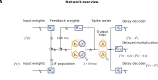
\includegraphics{media/chapters/04_temporal_tuning/spatio_temporal_overview.pdf}%
	\kern-158mm\includegraphics{media/chapters/04_temporal_tuning/spatio_temporal_overview_diagram.pdf}\\[0.5cm]
	\includegraphics{media/chapters/04_temporal_tuning/spatio_temporal_analysis.pdf}%
	{\phantomsubcaption\label{fig:spatio_temporal_a}}%
	{\phantomsubcaption\label{fig:spatio_temporal_b}}%
	{\phantomsubcaption\label{fig:spatio_temporal_c}}%
	{\phantomsubcaption\label{fig:spatio_temporal_d}}%
	\caption[Two-dimensional quantities over time in a rank one spatiotemporal network]{
		Two-dimensional quantities over time in a rank one spatiotemporal network.
		\textbf{(A)}~Overview of the network and results for some exemplary inputs $\mathfrak{x}_1(t)$ and $\mathfrak{x}_2(t)$.
		The input signals are fed into a recurrent network where each neuron is tuned to a random linear combination of the inputs, and a linear combination of the \LDN impulse responses for $q = 5$ and $\theta = \SI{1}{\second}$.
		%After filtering the output spike trains, we can decode linear and nonlinear functions over time and space.
		We can approximately decode delayed versions of the inputs (a linear transformation) and the product of the two input signals for $\theta_1 = \theta_2$.
		\textbf{(B)}~For band-limited noise inputs, delayed versions of the both input signal can be decoded with a small mean delay decoding error $\bar E$. Dashed lines are the delay decoding errors for an equivalent Echo State Network (\ESN; \cite{jaeger2004harnessing}).
		\textbf{(C)}~Decoding error (\NRMSE) when systematically decoding delayed multiplication for delays $\theta_1$, $\theta_2$.
		While the resulting error is quite large, it is substantially smaller than what is achievable with linear approximations of four-quadrant multiplication (i.e., an \NRMSE of $100\%$). Decoding delayed multiplication works best for $\theta_1 = \theta_2$.
		For an \ESN, all errors are above $100\%$.
		\textbf{(D)} Normalised singular values of the recurrent weight matrix.
		The matrix is of rank twelve, with the last four singular values being relatively small.
	}
	\label{fig:spatio_temporal}
\end{figure}

Results are depicted in \Cref{fig:spatio_temporal}.
It is possible to decode delayed versions of the individual input signals with similar errors as in previous experiments.
Decoding delayed multiplication generally results in relatively large errors, with a minimum error of $36\%$.
Most notably, errors are minimal along the diagonal, i.e., $\theta'_1 = \theta'_2$.

\paragraph{Discussion}
Decoding errors for off-diagonal $\theta'_1$, $\theta'_2$ pairs being large is due to $\mat E^\mathrm{t}$ being of rank one.
Each neuron is temporally tuned to a linear combination of the spatial input signal dimensions.
For example, for some $\vec e_i$, $\vec e_i^\mathrm{t}$, the neuron is most active if the time-course of the linear combination $\langle \vec e_i, \mathfrak{x}(t) \rangle$ is similar to the time-course described by the function $\langle \vec e_i^\mathrm{t}, \mathfrak{h}(t) \rangle$.

However, using rank one $\mat E_i^\mathrm{t}$, it is impossible to generate neural tuning such that a neuron is tuned to different input dimensions having different temporal behaviour.
As a result, we cannot decode functions that are nonlinear over several time-points.
This is similar to not being able to decode nonlinear functions from neuron populations with axis-aligned spatial encoders (cf.~\Cref{sec:two_layer_intermediate}).
We reach \NRMSEpl below $100\%$ for $\theta'_1 \neq \theta'_2$ when computing delayed multiplication because the product for the closest uniform delay is a decent approximation.


\subsubsection{Delayed multiplication with full rank $\mat E^\mathrm{t}$}

We repeat the above experiment with full rank spatiotemporal encoding matrices $\mat E^\mathrm{t}$.
That is, instead of sampling spatial and temporal encoding vectors $\vec e_i$, $\vec e^\mathrm{t}_i$, we generate random $\mat E^\mathrm{t}$ with Frobenius norm $\| \mat E^\mathrm{t} \|_\mathrm{F} = 1$.
Specifically, we uniformly sample vectors from the hypersphere $\mathbb{S}^{dq}$, and reshape these vectors into matrix form.

\paragraph{Results}

\begin{figure}
	\centering
	\includegraphics{media/chapters/04_temporal_tuning/spatio_temporal_analysis_matrices.pdf}%
	{\phantomsubcaption\label{fig:spatio_temporal_full_a}}%
	{\phantomsubcaption\label{fig:spatio_temporal_full_b}}%
	{\phantomsubcaption\label{fig:spatio_temporal_full_c}}%
	\caption[Decoding delayed multiplication in a network with full rank spatiotemporal encoders]{
		Decoding delayed multiplication in a network with full rank spatiotemporal encoders $\mat E_i^\mathrm{t}$.
		Same architecture as in \Cref{fig:spatio_temporal_a}.
		\textbf{(A)} Decoding delayed versions of the two input dimensions. Note the slightly smaller mean delay decoding error compared to using a rank one spatiotemporal encoding matrix.
		\textbf{(B)} Delayed multiplication decoding errors are approximately uniform for all combinations of $\theta_1$ and $\theta_2$.
		\textbf{(C)} The recurrent weight matrix now possesses $d q = 10$ non-zero singular values.
	}
	\label{fig:spatio_temporal_full}
\end{figure}

Errors for delay decoding and computing delayed multiplication are given in \Cref{fig:spatio_temporal_full}.
Note that the errors for decoding delayed versions of the individual input signals are slightly smaller than before (\Cref{fig:spatio_temporal_full_a}).
The results for computing delayed computation show a drastic improvement (\Cref{fig:spatio_temporal_full_b}).
Errors are between $30\%$ to $40\%$ for all $\theta'_1$, $\theta'_2$ pairs.

\paragraph{Discussion}
Improvements in the linear delay decoding task are due to a slight reduction in our solver loss from \cref{eqn:weight_optimise_currents_temporal}; the more diverse tuning facilitates realising the desired tuning in the recurrent connection.
The reduction in error for delayed multiplication is as expected.

Finally, note that the recurrent weight matrices are of low rank (\Cref{fig:spatio_temporal_d,fig:spatio_temporal_full_c}).
This suggests that it is possible to realise the same network in the \NEF without temporal tuning.
Indeed, as we show in \Cref{app:spatiotemporal_nef}, this is possible.
However, we must realise a $qd$-dimensional representation in the population; implementing dynamical systems with spiking neurons in such high dimensional spaces can be challenging.
Our approach offers the advantage of biasing the weight solver towards portions of the activity space relevant for certain input signals and thus results in smaller errors in the delayed multiplication task.

\subsubsection{Example: Recently travelled distance}

\begin{figure}
	\includegraphics{media/chapters/04_temporal_tuning/path_integration.pdf}
	\caption[Decoding the recently travelled distance distance from a spatiotemporal network]{Decoding the recently travelled distance distance from a spatiotemporal network. Same experimental setup as in \Cref{fig:spatio_temporal}, but decoding the distance travelled over the past second instead.
	\textbf{(A)} Random trajectory generated by integrating the input velocities in $x_1$- and $x_2$-direction.
	Highlighted section (black line and coloured circles) corresponds to the time range displayed in \emph{(B)}.
	\textbf{(B)} Input velocities $\dot x_1(t)$ and $\dot x_2(t)$ and the decoded windowed distance $d_{[t - \theta, t]}$.
	Dotted line is the ground-truth. The \NRMSE $E$ is computed after subtracting the mean (without subtracting the mean $E = 8.1\%$).
	Again, \NRMSEpl are far above $100\%$ when using an \ESN (grey dashed line).
	}
	\label{fig:path_integration}
\end{figure}

As a slightly more practical example of a function that could be decoded from a spatiotemporal network, consider the distance an agent has travelled over the past $\theta$ seconds.
For the sake of simplicity, let $\dot x_1(t)$, $\dot x_2(t)$ denote the velocity of the agent in a global coordinate space.
We define the \emph{recently travelled distance} $d_{[t - \theta, t]}$ as
\begin{align*}
	d_{[t - \theta, t]}(\dot x_1, \dot x_2) = \int_{t - \theta}^t \sqrt{\dot x_1(\tau)^2 + \dot x_2(\tau)^2} \,\,\mathrm{d}\tau \,.
\end{align*}

We test decoding this function using the spike data recorded in the experiment with rank one $\mat E_i^\mathrm{t}$.
Results are depicted in \Cref{fig:path_integration}.
We obtain an \NRMSE of $E \approx 22\%$ over $T = \SI{100}{\second}$.
Interestingly, using the full rank $\mat E_i^\mathrm{t}$ we obtain $E \approx 26\%$ (data not shown).

\paragraph{Discussion}
This experiment indicates that it can be beneficial to restrict the encoders to a lower rank.
We apply a linear operator (the integral) to a function that is only nonlinear over the same point in time $\tau$---this is exactly the type of function supported by our rank one spatiotemporal encoding matrices.

Overall, our experiments demonstrate that it is possible to realise populations with spatiotemporal tuning in the \NEF; our \emph{spiking} networks even outperform the popular non-spiking Echo State Network (\cite{jaeger2004harnessing}) by a wide margin.
A next step would be to use this technique to construct a neurophysiologically motivated model of spatiotemporal tuning.

\pagebreak

\subsection{Adaptive Filters}
\label{sec:adaptive_filter}

Another interesting application of neural networks with spatiotemporal tuning is using them to construct nonlinear \emph{adaptive filters}.
Here, we discuss an adaptive variant of the Wiener filter \citep[Chapter~2]{wiener1949extrapolation,haykin2014adaptive}.
\emph{Adaptive} refers to updating the usually static filter parameters on-the-fly, in response to an error signal $\epsilon(t)$ while the system is operating.
This is in principle comparable to learning and adaptation in animals.

The core idea of Wiener filters is to linearly combine filtered versions of an input signal with the goal of minimising a linear least-squares loss.%
\footnote{Notably, Wiener provides conditions under which an optimal $\vec d$ can be obtained.
\Citet{kalman1960new} broadens the optimality conditions by accounting for uncertainty and proposing an optimal update rule.}
Let $h_i(t)$ be one of $n$ filter kernels, $\vec d = (d_1, \ldots, d_n)$ a set of weights, $\mathfrak{u}(t)$ an input signal, and $\mathfrak{x}(t)$ a desired output signal.
Then, in the simplest case, this optimisation problem can be stated as follows:
\begin{align}
	E = \left( \int_0^T \!\! \mathfrak{x}(t) - \sum_{i = 1}^n d_i \, (\mathfrak{u} \ast h_i)(t) \, \mathrm{d}t \right)^2
	\! = \left( \int_0^T \!\! \mathfrak{x}(t) - \sum_{i = 1}^n d_i a_i(\mathfrak{u} \ast \delta_{-t}) \, \mathrm{d}t \right)^2 \,.
	\label{eqn:wiener}
\end{align}
where, as in \cref{eqn:weight_optimise_currents_temporal}, $\delta_{-t}$ is a shifted Dirac delta, and $a_i(\mathfrak{u}) = (\mathfrak{u} \ast h_i)(0)$.

As pointed out by \Citet{wiener1949extrapolation}, this kind of optimisation problem can be interpreted in multiple ways, two of which are compatible with adaptation.
First, \cref{eqn:wiener} can be used to find $\vec d$ that extract \enquote{hidden} information $\mathfrak{x}(t)$ from $\mathfrak{u}(t)$ by removing unwanted noise---hence the term \emph{filter}.
Wiener refers to this as \emph{interpolation}.
Second, if $\mathfrak{x}(t)$ corresponds to a future point in time relative to $\mathfrak{u}(t)$, then these equations can be used for \emph{prediction} or \emph{extrapolation}.

Now, to adapt $\vec d$ over time, we take the gradient of $E$ in \cref{eqn:wiener} with respect to $\vec d$ for the current signal history $\mathfrak{u} : \mathbb{R}^- \longrightarrow \mathbb{R}$ and perform gradient descent over time:
\begin{align}
	\frac{\partial}{\partial d_i(t)} E \propto \left(y(t) - \sum\nolimits_{i = 1}^n d_i(t) \, a_i(\mathfrak{u}) \right) a_i(\mathfrak{u}) = \epsilon(t) a_i(\mathfrak{u}) \quad\quad \leadsto \quad\quad \dot{d}_i(t) = - \eta \epsilon(t) a_i(\mathfrak{u}) \,.
	\label{eqn:delta_rule}
\end{align}
Here, $\epsilon(t)$ is the momentary error, and $\eta$ is a learning rate.
Crucially, instead of setting $a_i$ to a linearly filtered version of $\mathfrak{u}$, we can use the activities $a_i$ of a nonlinear neural network with temporal tuning.
In this case, \cref{eqn:delta_rule} is the \emph{delta learning rule}, a precursor to back\-pro\-pa\-ga\-tion that has been developed with nonlinear adapitve filters in mind \citep{widrow1960adaptive}.%
\footnote{For nonlinear neurons, we have to multiply \cref{eqn:delta_rule} by a gradient term $a_i'$. We typically ignore this for \LIF neurons, which, if not saturated, resemble \ReLUpl. Correspondingly, $a_i'$ is a constant factor if the neuron is active.}

\Citet{macneil2011finetuning} propose a biologically plausible version of \cref{eqn:delta_rule} that can be integrated into spiking neural networks.
We discuss this Prescribed Error Sensitivity (\PES) rule in more detail in \Cref{sec:cerebellum_eyeblink}.
For now, we would like to demonstrate that the combination of our spatiotemporal spiking \NEF populations and the delta rule results in a powerful adaptive filter that can, for example, learn to predict the nonlinear dynamics of a forced pendulum over time.
Forced pendulums are found in most robotic actuators and can, under some conditions, exhibit chaotic behaviour \citep{hubbard1999forced}.

\subsubsection{Methods}

\begin{figure}
	\centering
	\includegraphics{media/chapters/04_temporal_tuning/04_03/pendulum_overview.pdf}
	\includegraphics{media/chapters/04_temporal_tuning/04_03/pendulum_examples.pdf}%
	{\phantomsubcaption\label{fig:pendulum_overview_a}}%
	{\phantomsubcaption\label{fig:pendulum_overview_b}}%
	{\phantomsubcaption\label{fig:pendulum_overview_c}}%
	\caption[An adaptive filter learning pendulum dynamics]{
		An adaptive filter learning pendulum dynamics.
		\textbf{(A)} Illustration of the nonlinear pendulum system.
		A point mass $m = \SI{1}{\kilogram}$ under the influence of gravity $\| \vec g \| = \SI{9.81}{\metre\per\square\second}$ is connected to a rotating joint through a rigid rod of length $L = \SI{1}{\metre}$.
		A random torque $\tau(t)$ is applied to the joint; we measure the angle of the pendulum $\phi(t)$.
		\textbf{(B)} The angle $\tau(t)$ and a delayed version of the angle $\phi(t - \theta')$ are fed into the full-rank spatiotemporal \NEF network from the previous subsection.
		After passing the spikes through a short low-pass filter, we decode the angle at time $t$ using a decoding vector $\vec d$.
		This decoding matrix is updated according to the delta rule; the network \emph{learns} the nonlinear pendulum dynamics.
		\textbf{(C)}~Examples of the pendulum dynamics and prediction after different amounts of training.
	}
	\label{fig:pendulum_overview}
\end{figure}
As is depicted in \Cref{fig:pendulum_overview}, we apply a low-pass filtered white noise signal $\tau(t)$ as a torque to the rotational joint of a simulated pendulum.%
\footnote{We use our library \emph{PyKinSim} (\url{https://github.com/astoeckel/pykinsim}) as a kinematic chain simulator.}
Care has been taken to choose the frequencies and amplitude of $\tau(t)$ such that the pendulum regularly switches between a resonance mode---where the pendulum merely oscillates with its approximate resonance period $2 \pi \sqrt{L g^{-1}}$---and a mode where the pendulum is more directly influenced by $\tau(t)$.
These modes are to some degree visible in the two rightmost plots of \Cref{fig:pendulum_overview_c}.

Our spatiotemporal neuron population from the last subsection ($d = 2$, $q = 5$, $n = 1000$) receives both the torque $\tau(t)$ and a time-delayed version of the pendulum joint angle $\phi(t - \theta')$, where $\theta' = \SI{0.75}{\second}$.
Inputs to the network are rescaled to the interval $[-1, 1]$.

\pagebreak

We autoregressively learn a decoding vector $\vec d$ using \cref{eqn:delta_rule} and the error signal $\epsilon(t) = \phi(t) - \hat \phi(t)$, where $\hat \phi(t)$ is the decoded and low-pass filtered spiking activity.
Since the input angle $\phi(t - \theta')$ is delayed, the system essentially learns to \emph{predict} the motion of the pendulum $\theta'$ seconds into the future given the future torque trajectory.
We set the learning rate $\eta$ to $\num{2e-4}$ and train over $\SI{1000}{\second}$.%
\footnote{Larger learning rates---and shorter simulation times---are possible, but our setup generates enough data to construct a relatively noise-free learning curve, i.e., \Cref{fig:pendulum_overview_c}.}

As a control experiment, we test only feeding one of the input dimensions---that is, either the angle $\phi(t - \theta')$ or the torque $\tau(t)$---into the system.
This way, we can ensure that the predicted dynamics indeed depend on both the past pendulum state and the torque; for example, the torque $\tau(t)$ is mostly irrelevant if the pendulum is in its resonance mode.

\subsubsection{Results}

\begin{figure}
	\centering
	\includegraphics{media/chapters/04_temporal_tuning/04_03/pendulum_error_plots.pdf}
	\caption[Adaptive filter error over time]{
		Adaptive filter error over time.
		Area right to the black dashed line is without adaptation.
		\textbf{(A)} Error signal $\epsilon(t)$ over time; dark line is a low-pass filtered version.
		\textbf{(B, C)} Control experiment where only one of the two input dimensions are available to the network.
		Evidently, both are necessary to compute the function well.
		\textbf{(D)} Same data as before, but as \NRMSE over bins of length $\SI{50}{\second}$.
	}
	\label{fig:pendulum_error_plots}
\end{figure}

Examples of the inputs and the predicted output are depicted in \Cref{fig:pendulum_overview_c}.
A more thorough analysis of the error $\epsilon(t)$ over time is provided in \Cref{fig:pendulum_error_plots}.
Generally, the phase of the prediction is correct, but the amplitude of the peaks is often slightly over- or under-estimated.
The final \NRMSE reached by the network is about $20\%$.
Our control experiments show that both $\tau(t)$ and $\phi(t - \theta')$ critically contribute to the prediction.

\subsubsection{Discussion}

Our nonlinear adaptive filter learns to predict the nonlinear pendulum dynamics reasonably well.
Possible sources for error are the relatively small $q$, the limited neural resources, and the remaining spike noise.
Interesting future work includes exploring the relationship between this kind of adaptive filter and hierarchical pedictive coding networks based on a more general formalisation of Kalman filtering \citep{bastos2012canonical}.
We discuss adaptive filters in the context of a biologically constrained model of the cerebellum in \Cref{chp:cerebellum}.

\clearpage

\subsection{Accounting for Intrinsic Neural Dynamics}
\label{sec:temporal_tuning_neural_dynamics}

So far, we have focused on synaptic filters as the primary temporal resource in spiking neural networks.
However, as we mentioned several times throughout this thesis, neurons themselves can be a significant source of dynamics.
Our temporal tuning approach suggests a way to account for neural dynamics while solving for weights; however, this is by no means a one-size-fits-all solution for every neuron model.
Below, we discuss the abstract optimisation problem, point out solution strategies, and demonstrate that we can account for \ALIF dynamics.

\subsubsection{Optimisation problem}
Remember that our temporal tuning paradigm assigns tuning properties to each neuron $i$---given some input signal $\mathfrak{x}_k$, we define a desired output rate $a_i(\mathfrak{x}_k)$.
Under the assumption that the pre-neurons $j$ adhere to their normative tuning, we then solve for weights $w_{ij}$ that decode a current $J_i(\mathfrak{x}_k)$ evoking the desired rate.
The mapping between currents and rates is according to a \emph{static} response curve $G[J]$; it holds $a_i(\mathfrak{x}_k) = G[J_i(\mathfrak{x}_k)]$.

If we would like to account for intrinsic neural dynamics, then we can no longer assume static response curves.
Instead, we must model the average firing rate of a neuron depending on its input current history; we have a \emph{temporal} response curve $\Omega[\mathfrak{J}] : (\mathbb{R}^- \longrightarrow \mathbb{R}) \longrightarrow \mathbb{R}^+$, where $\mathfrak{J}$ is a signal describing the past post-synaptic currents, and $\Omega[\mathfrak{J}]$ is the rate at $t = 0$.

Since our weight optimisation problem is in current space, we need to map from the rate determined by the tuning curve $a_i(\mathfrak{x}_k)$ onto a current.
More precisely, we search for a function of the form $\Omega^{-1}[\mathfrak{a}] : (\mathbb{R}^- \longrightarrow \mathbb{R}^+) \longrightarrow \mathbb{R}$:%
\footnote{Note that we write $\Omega^{-1}$ only for notational purposes; this is not strictly speaking the mathematical inverse of $\Omega$.
Since $\Omega$ is unlikely to be bijective, $\Omega^{-1}$ is ill-defined.
Furthermore, having $\Omega^{-1}$ only depend on the output history may not be sufficient for complex neuron models; the entire input history may play a role in determining the \enquote{correct} input current.
It is unclear how this could be incorporated into our optimisation problem.
}
given a desired output rate signal $\mathfrak{a}$, this function returns the post-synaptic current $J$ that should be injected into the neuron in the present, at $t = 0$.
Consequently, our optimisation problem in \cref{eqn:weight_optimise_currents_temporal} becomes
\begin{align}
	E = \sum\nolimits_{k = 1}^N \Bigl[
		\Omega^{-1}[\mathfrak{a}_i(f(\mathfrak{x}_k)] -
		\!\sum\nolimits_{j = 1}^m w_{ij} (h_{ij} \! \ast \! \mathfrak{a}_j(\mathfrak{x}_k))(0) \,\mathrm{d}\tau
	\Bigr]^2 \!, \;\;
	\text{where} \; (\mathfrak{a}_i(\mathfrak{x}_k))(t) = a_i(\mathfrak{x}_k \! \ast \! \delta_{-t}) \,.
	\label{eqn:weight_optimise_currents_temporal_nonlin}
\end{align}
While this optimisation problem is still in linear least-squares form, $\Omega^{-1}$ is typically a rather complex spatiotemporal function.
Correspondingly, we can only expect to solve \cref{eqn:weight_optimise_currents_temporal_nonlin} with a small error if the pre-population tuning forms an expressive spatiotemporal function basis.

Determining $\Omega^{-1}$ is generally difficult, and, for most neuron models, a research project of its own.
One approach explored by \citet{hunsberger2016system} is to employ linear-nonlinear models of the form $\Omega[\mathfrak{J}] = G[(\mathfrak{J} \ast \mathfrak{h})(0)]$.
In this case, we do not necessarily have to use \cref{eqn:weight_optimise_currents_temporal_nonlin}, but can simply treat $\mathfrak{h}$ as an additional filter next to the $h_{ij}$ in \cref{eqn:weight_optimise_currents_temporal}; this will implicity solve for $\Omega^{-1}$.

The following is another method for implicitly determining $\Omega^{-1}$---however, as of writing, this still requires further investigation.
The basic idea is to iteratively compensate for errors introduced by the intrinsic neural dynamics.
That is, after solving for weights as in \cref{eqn:weight_optimise_currents_temporal}, we can determine the actual population response $\hat a_i(\mathfrak{x}_k)$ for synthetic pre-population spike trains that perfectly follow the desired tuning $\mathfrak{a}_j(\mathfrak{x}_k)$ (cf.~\Cref{fig:alif_a}).
Using the deviation from the desired output rate $\epsilon_{ik} = \hat a_i(\mathfrak{x}_k) - a_i(\mathfrak{x}_k)$, we estimate an offset current $J_{ik}$ that compensates for $\epsilon_{ik}$.
We add this $J_{ik}$ to \cref{eqn:weight_optimise_currents_temporal}, solve for new weights, and repeat.
This is similar to an approach described by \citet{duggins2017incorporating} that has been successfully applied to biologically detailed neurons.

\subsubsection{Accounting for \ALIF dynamics}
$\Omega^{-1}(\mathfrak{a})$ is readily available for the adaptive leaky integrate-and-fire model (\ALIF).
The \ALIF model accounts for firing-rate adaptation observed in biological neurons (cf.~\Cref{fig:izhikevich_whichmod_figure1f}) by increasing an exponentially decaying adaptation variable $n(t)$ by a constant amount $n_0$ every time the neuron spikes \citep{treves1993meanfield}.
The specific \ALIF model discussed here applies this spike-triggered adaptation mechanism to a current-based \LIF neuron by subtracting the adaptation variable $n(t)$ from the input current $J(t)$.
Despite its simplicity, this model can be made to fit empirical spike data from cortical pyramidal cells well \citep{camera2004minimal}.

\begin{figure}
	\includegraphics{media/chapters/04_temporal_tuning/04_03/alif_dynamics.pdf}%
	{\phantomsubcaption\label{fig:alif_a}}%
	{\phantomsubcaption\label{fig:alif_b}}%
	\caption[Accounting for ALIF dynamics]{
		Accounting for \ALIF dynamics.
		\emph{Left:} Recurrent network implementing a \SI{2}{\hertz} oscillator with $100$ \LIF neurons (maximum rates at \SI{200}{\per\second}).
		\emph{Middle:} Same network with \ALIF neurons; not taking dynamics into account.
		\emph{Right:} Compensating for the \ALIF dynamics.
		\textbf{(A)} Comparison between the actual response $\hat{\mathfrak{a}}_i(\mathfrak{x}_k)$ of a neuron $i$ for the $k$th sample $\mathfrak{x}_k$ to the expected response $\mathfrak{a}_i(\mathfrak{x}_k)$.
		The neuron receives synthetic spike trains matching the expected pre-population rates.
		\textbf{(B)} Decoded system state of the freely running network. Without compensation, the low-pass dynamics of the \ALIF neuron cause a rapid decay; with compensation the network behaves as expected.
	}
	\label{fig:alif}
\end{figure}

To account for \ALIF dynamics within \cref{eqn:weight_optimise_currents_temporal_nonlin}, we merely need to decode the adaptation current from the pre-population.
Given the adaptation decay time-constant $\tau_\mathrm{n}$, we have
\begin{align*}
	\Omega^{-1}(\mathfrak{a}) &= G^{-1}[\mathfrak{a}(0)] + n_0 (\mathfrak{a} \ast h_\mathrm{n})(0) \,, & \text{where } h_\mathrm{n}(t) = \tau_\mathrm{n}^{-1} \exp(-t \tau_\mathrm{n}) \,,
\end{align*}
and where $G^{-1}[a]$ is the current required to evoke a rate $a$ according to the static \LIF model.
We demonstrate successfully accounting for \ALIF dynamics ($\tau_\mathrm{n} = \SI{100}{\milli\second}$, $n_0 = \SI{0.01}{\nano\ampere}$) in this way in \Cref{fig:alif}.
The only requirement for this to work is that the pre-population forms a temporal basis from which $h_\mathrm{n}$ can be decoded.
In a sense, if we tune our neurons to possess low-pass dynamics, then this approach allows us to \emph{harness} the \ALIF dynamics---after all, the \ALIF neuron intrinsically implements a low-pass filter (cf.~\Cref{fig:neural_dynamics_firing_rates}).